\documentclass{ltjbook}
\usepackage{docmute} 
\usepackage{../../myStyle} 

\begin{document}
\chapter{群間計画(Between Design)と分散分析}
\label{ch18_BetweenDesign}

実験計画について，用語の整理や効果の評価の方法について説明してきました。前回は一要因の実験計画でしたが，今回はこれを二要因に増やした場合について考えていきます。

\section{群間計画の基本構造}
\label{Between2way}
今度は，二要因の群間計画に進んでいきたいと思います。
二要因計画とはたとえば，次のような実験計画です。

\begin{quote}
	植物の生長を観察するため，水をあげる群とあげない群，肥料をあげる群とあげない群をつくり，成長の程度を比較したい
\end{quote}

この例では要因は「水」と「肥料」，水準はそれぞれ「あげる・あげない」なので$2\times2$の実験計画というのでした。

アサガオの例のまま進めても良いのですが，もう少し心理学っぽいほうがイメージしやすいかもしれませんので，以下では表\ref{tbl:18_01}のようなコーヒーテイスティング事例を使うことにします。

2つのメーカーがそれぞれ缶コーヒーを作っていて，ホットコーヒーにした場合，アイスコーヒーにした場合の美味しさを評価してもらいます。各条件に3名ずつ試飲をお願いして，20点満点で評価してもらったら，表\ref{tbl:18_01}のようになりました\footnote{添字にカンマが入っているのが美しくないですね。しかし他の良い方法が思いつきませんでした。}。これを図示したのが図\ref{fig:18_01}にあります。
これを見るとわかるように，ホットコーヒーにすると銘柄Aは高い評価，アイスコーヒーだと両者の違いはなくなることがわかります。
どうも銘柄Bはホットコーヒーにして売らない方がいいように思いますが，たまたまホットの銘柄Bを飲んだ3人がコーヒーが苦手だったのかもしれませんね。
このような誤差に比べて，温度と銘柄の別の効果はどの程度あるのかを考えていきたいと思います。
% latex table generated in R 4.0.2 by xtable 1.8-4 package
% Fri Sep 11 14:11:29 2020
\begin{table}[ht]
	\centering
	\caption{二要因のデータ例}
	\begin{tabular}{rrrcr}
		\hline
		ID & 温度   & メーカー & notation                  & 評価($y_{i}$) \\
		\hline
		1  & Hot  & 銘柄A  & $X_{11}=+1,X_{12}=+1$     & 13          \\
		2  & Hot  & 銘柄A  & $X_{21}=+1,X_{22}=+1$     & 11          \\
		3  & Hot  & 銘柄A  & $X_{31}=+1,X_{32}=+1$     & 12          \\
		4  & Hot  & 銘柄B  & $X_{41}=+1,X_{42}=-1$     & 7           \\
		5  & Hot  & 銘柄B  & $X_{51}=+1,X_{52}=-1$     & 6           \\
		6  & Hot  & 銘柄B  & $X_{61}=+1,X_{62}=-1$     & 8           \\
		7  & Cold & 銘柄A  & $X_{71}=-1,X_{72}=+1$     & 9           \\
		8  & Cold & 銘柄A  & $X_{81}=-1,X_{82}=+1$     & 9           \\
		9  & Cold & 銘柄A  & $X_{91}=-1,X_{92}=+1$     & 9           \\
		10 & Cold & 銘柄B  & $X_{10,1}=-1,X_{10,2}=-1$ & 13          \\
		11 & Cold & 銘柄B  & $X_{11,1}=-1,X_{11,2}=-1$ & 11          \\
		12 & Cold & 銘柄B  & $X_{12,1}=-1,X_{12,2}=-1$ & 9           \\
		\hline
	\end{tabular}

	\label{tbl:18_01}
\end{table}

\begin{figure}[ht]
	\centering
	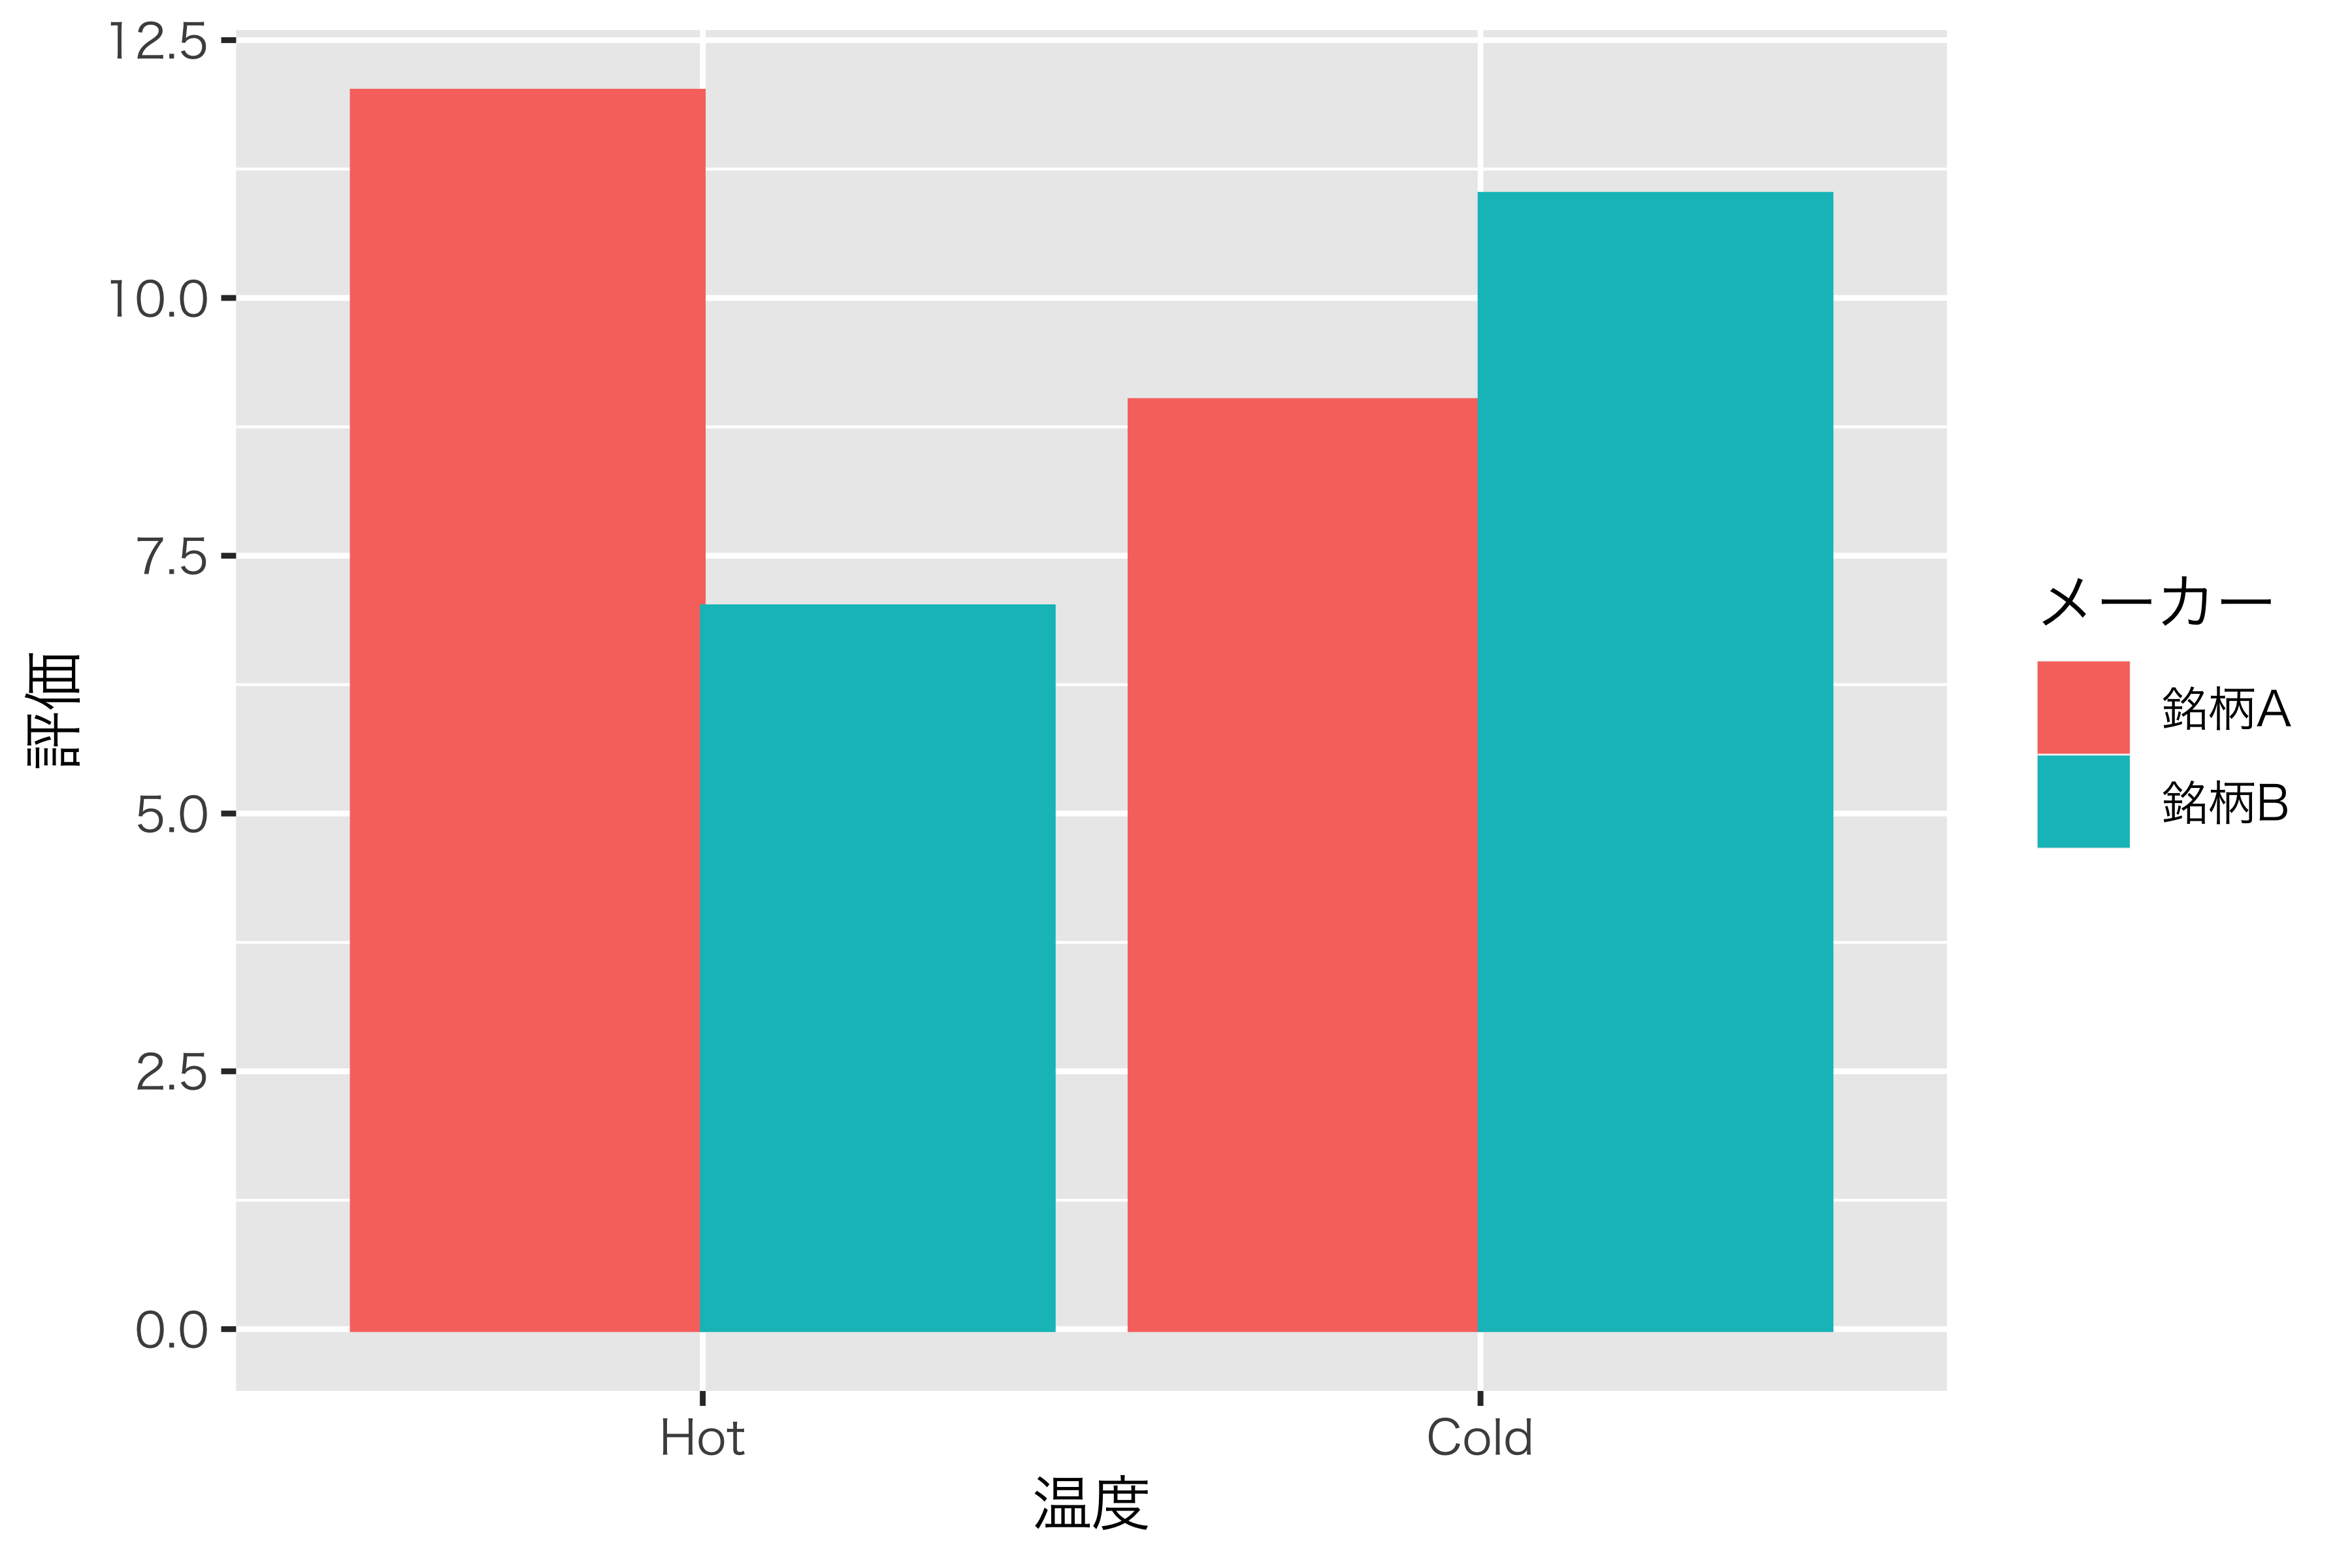
\includegraphics[keepaspectratio,width=0.8\linewidth]{figures/18_BetweenDesign/BetweenDesign1.png}
	\caption{2種類のコーヒーと2通りの飲み方による評価}
	\label{fig:18_01}
\end{figure}

さて，一要因の計画は，線形モデルと見ることができるという話をしていました。
二要因の計画も当然，同じように線形モデルとして考えることができます。今回は二要因計画です。要因は「温度」と「銘柄」の二種類ありますから，効果として$b_1$と$b_2$の2つが必要です。これを式に書き入れてみますと，次のようになります。
\begin{equation}
	\label{eq18_01}
	y_{i} = b_0 + b_1 X_{i1}+ b_2 X_{i2} + e_{i}
\end{equation}

ここで左辺の$y_{i}$はIDが$i$の人の評価で，たとえば$y_1=13,y_2=11,\cdots,y_{12}=9$ということになります。
$X_{ij}$は$i$さんが要因$j$のときにどちらに割り振られたかを表しているのだと思ってください。$j=1$は温度の要因，$j=2$は銘柄の要因を表しています。ですから，$X_{i1}$は$i$さんが温度要因でHot/Coldのどちらを飲んだかを表します。具体的には，$X_{11}$はHot条件です。$X_{71}$ はCold条件です。これは\keytermL{名義尺度水準}{めいぎしゃくどすいじゅん}であり，Hot/Coldになんらかの数字を割り振らなければなりません。数字は何でもいいといえば何でもいいのですが，ここでは数式的にわかりやすくするためにHotに+1を，Coldに-1を割り振ることにします。こうすることで，$b_1$が温度効果の大きさを表すことになりますね。Hot/Coldで符号が違って大きさが同じですから，相対的な大きさを表しているだけになるからです\footnote{他にもHotを0,Coldを1とすることもできます。するとHot条件を基準にしたCold条件の変化の大きさを表したことになります。詳しくは次講で扱います。}。$X_{11}=+1,X_{71}=-1$のような数字が入るものだと思って読み進めてください。同様に，$X_{i2}$は銘柄水準の割当を表していて，銘柄Aは+1,銘柄Bは-1を表しています。具体的に書き起こしてみましょう。


\[
	\label{eq18_02}
	\left \{
	\begin{array}{cccccc}
		y_1    & = & b_0 + b_1 X_{11} + b_2 X_{12} + e_1        & = & b_0 + b_1 + b_2 + e_1    & \mbox{Hotで銘柄A}  \\
		\vdots &   & \vdots                                     &   & \vdots                   &                 \\
		y_4    & = & b_0 + b_1 X_{41} + b_2 X_{42} + e_4        & = & b_0 + b_1 - b_2 + e_4    & \mbox{Hotで銘柄B}  \\
		\vdots &   & \vdots                                     &   & \vdots                   &                 \\
		y_7    & = & b_0 + b_1 X_{71} + b_2 X_{72} + e_7        & = & b_0 - b_1 + b_2 + e_7    & \mbox{Coldで銘柄A} \\
		\vdots &   & \vdots                                     &   & \vdots                   &                 \\
		y_{10} & = & b_0 + b_1 X_{10,1} + b_2 X_{10,2} + e_{10} & = & b_0 - b_1 - b_2 + e_{10} & \mbox{Coldで銘柄B} \\
		\vdots &   & \vdots                                     &   & \vdots                   &                 \\
	\end{array}
	\right.
\]

ここで$X_{ij}$は符号だけを表している名義尺度水準であることを確認しておいてください。

改めて式\ref{eq18_01}や式\ref{eq18_02}を見ると，これも線形モデル，とくに説明変数が複数ある\keytermL{重回帰分析}{じゅうかいきぶんせき}のモデルと同じ形をしているのが分かりますね。重回帰分析は第\ref{ch08_MultipleRegression}講でやりましたが，そのモデル式と同じ形をしているのが確認できると思います。要因計画は線形モデルなのです。


\section{平方和の分解と変動の源泉}

それでは，効果の大きさ，誤差の大きさを見積もってみましょう。二要因の場合でも考え方は同じです。
無作為に割り当てたのですから，人間の手を加えなかったらデータの散らばりのすべては誤差(個体差)です。誤差はキャンセルし合うはずなので，理論的にはすべて平均値に一致するはずです。

しかし，やれ温度の操作だとか，やれメーカーの違いだとかで人によって違う介入があり，しかも人間のやることですので個人差も加わってしまいました。だからデータがばらついてしまったのだ，と考えるのです。

理想的には全部同じはずと考えると，実験もしなければ個人差もない，理想的なデータの値は全体平均$\bar{X}_{gm} = 9.75$にぴったり合致するはずなのでした。しかしそこに温度の効果$b_1$が関係してきます。図\ref{fig:18_02}の左にあるように，温度で群わけしてHot群だけの平均を計算してみましょう。
\[ \bar{y}_{H} = \frac{1}{6}\sum_{i=1}^6 y_i = \frac{1}{6} (13+11+12+7+6+8)= 9.5 \]
同じく，Cold群だけの平均は次のようになります。
\[ \bar{y}_{C} = \frac{1}{6}\sum_{i=7}^{12}y_i = \frac{1}{6}(9+9+9+13+11+9) = 10.0 \]
ここで，群平均-全体平均=効果だと考えられますから，Hot群に割り当てられると$-0.25$の効果が，Cold群に割り当てられると$+0.25$の効果があったということになります。

同様に，メーカーの効果も考えましょう。温度の効果を潰して(温度の効果で分けずに)銘柄Aのデータだけ取り出して，平均値を計算してみます\footnote{この数式の美しくないこと！$\sum$の中身が2つに分裂してしまっています。しかしこれは$i$を通し番号でつけたから仕方のないこと。ここでは$i$がIDをあらわしていますから，その何番目から何番目までが加算されているかを確認してください。}。
\[ \bar{y}_{A} = \frac{1}{6}\left(\sum_{i=1}^3y_{i} + \sum_{i=7}^9y_i \right)= \frac{1}{6}(13+11+12+9+9+9) = 10.5 \]
同様に，銘柄Bの平均値を計算します。
\[ \bar{y}_{B} = \frac{1}{6}\left(\sum_{i=4}^6y_i + \sum_{i=10}^{12}y_i \right) =\frac{1}{6}(7+6+8+13+11+9)= 9.0 \]

群平均-全体平均=効果ですから，銘柄Aは全体平均より$10.5-9.75=0.75$高くなる効果が，相対的に銘柄Bは全体平均より$0.75$下がる効果がある($-0.75$あげる効果がある)，ということがわかります。

図\ref{fig:18_02}に，群ごとに平均値をプロットし，全体平均(9.75)のラインを横一線で引いてみました。これを見ると，各群の効果が全体平均($b_0$)を挟んで，相対的に同じ大きさで影響しているのがわかると思います。
\begin{figure}[ht]
	\centering
	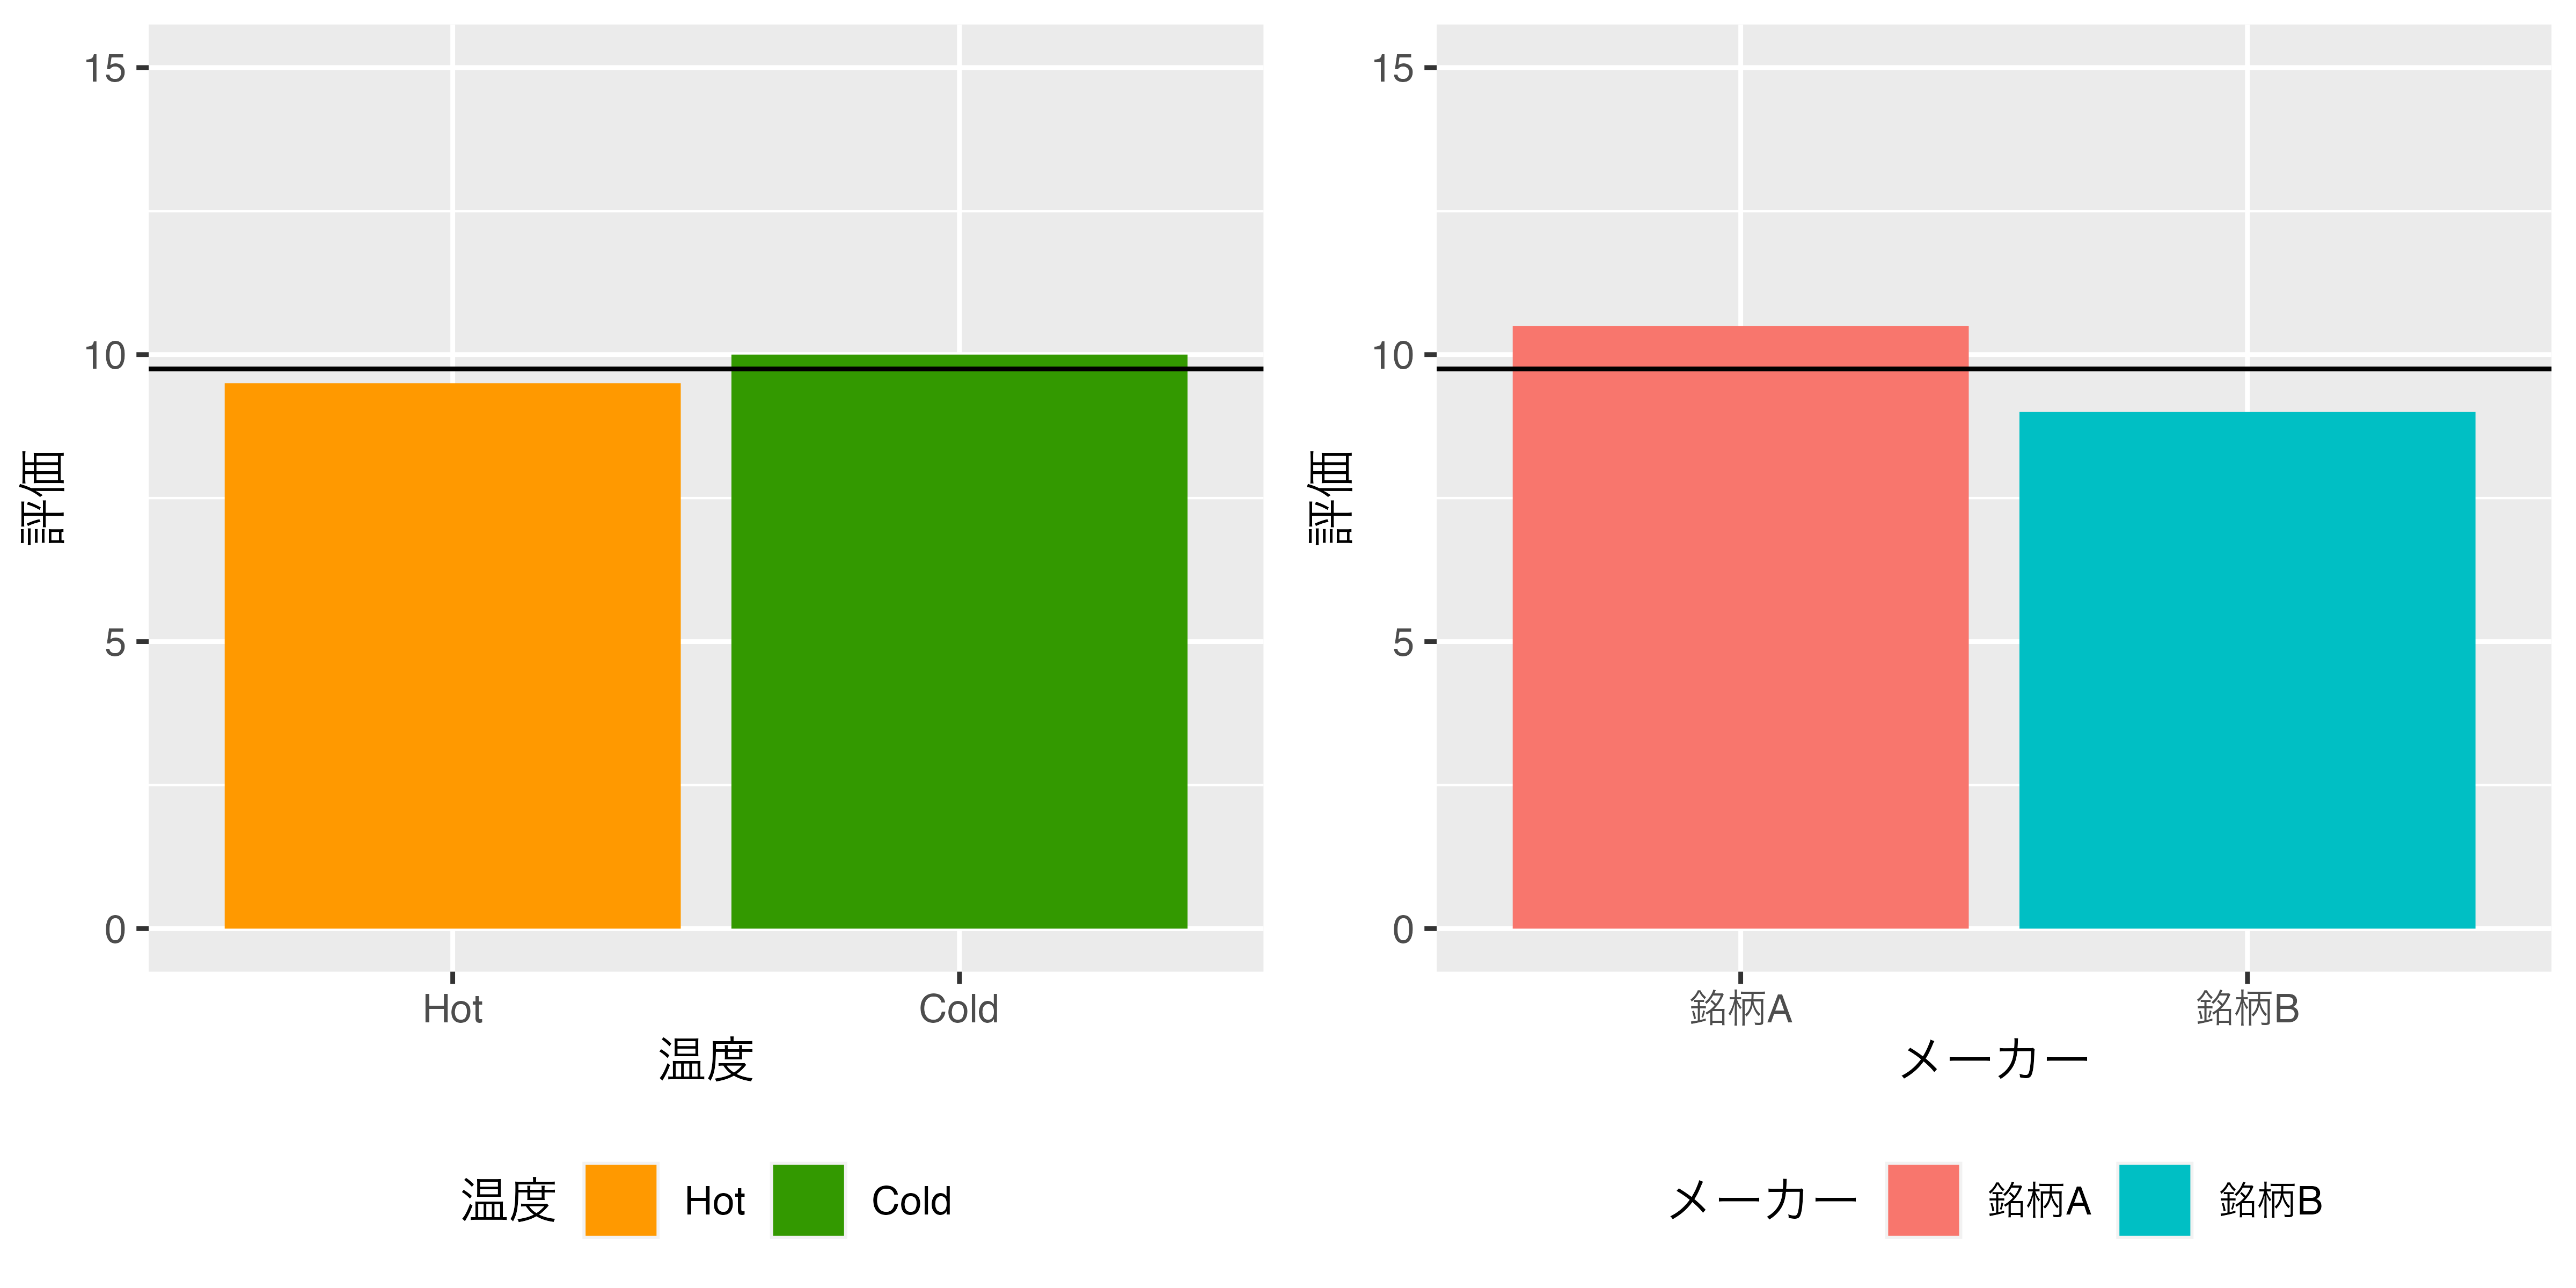
\includegraphics[keepaspectratio,width=0.8\linewidth]{figures/18_BetweenDesign/BetweenDesign2.png}
	\caption{群ごとにプロットしたもの。全体平均から見た相対評価になっていることが確認できる。}
	\label{fig:18_02}
\end{figure}

さて，これらの効果がわかったところで，足し算を組み上げていきましょう。全体平均にそれぞれの効果を加えていきます。銘柄Aをホットコーヒーでいただくとすると，全体平均$ 9.75$にHotの効果があって($-0.25$)の銘柄Aの効果($+0.75$)も入りますから，$9.75-0.25+0.75=10.25$となり，これが銘柄Aをホットで飲んだ時の平均値になるはずですが・・・

\[ \bar{y}_{H,A} = \frac{1}{3}\sum_{i=1}^3 y_i =  \frac{1}{3}(13+11+12)=12 \]

あれ？ なりませんでした。

\section{交互作用の理解と解釈}
\label{interaction}
\subsection{交互作用の算出}
実は，同様のことは他の組み合わせのところでも生じます。群平均からの差分が誤差なのだ，と考えれば良いはずですが，群平均が理論通りにならないのです。具体的に，表\ref{tbl:18_02}に計算してみました。効果の総和と群平均，理論的には合致するはずです。これはどうしたことでしょう。
\begin{table}[ht]
	\centering
	\caption{二要因のデータ例}
	\begin{tabular}{rrrccr}
		\hline
		全体平均 & 温度の効果 & メーカーの効果 & 効果を足し合わせると              & 群平均は                  & 評価 \\
		\hline
		9.75 & -0.25 & +0.75   & \multirow{3}{*} {10.25} & \multirow{3}{*}{12.0} & 13 \\
		9.75 & -0.25 & +0.75   &                         &                       & 11 \\
		9.75 & -0.25 & +0.75   &                         &                       & 12 \\ \hline
		9.75 & -0.25 & -0.75   & \multirow{3}{*} {8.75}  & \multirow{3}{*}{7.0}  & 7  \\
		9.75 & -0.25 & -0.75   &                         &                       & 6  \\
		9.75 & -0.25 & -0.75   &                         &                       & 8  \\ \hline
		9.75 & +0.25 & +0.75   & \multirow{3}{*} {10.75} & \multirow{3}{*}{9.0}  & 9  \\
		9.75 & +0.25 & +0.75   &                         &                       & 9  \\
		9.75 & +0.25 & +0.75   &                         &                       & 9  \\ \hline
		9.75 & +0.25 & -0.75   & \multirow{3}{*} {9.25}  & \multirow{3}{*}{11.0} & 13 \\
		9.75 & +0.25 & -0.75   &                         &                       & 11 \\
		9.75 & +0.25 & -0.75   &                         &                       & 9  \\
		\hline
	\end{tabular}
	\label{tbl:18_02}
\end{table}

銘柄A($+0.75$)のホットコーヒー($-0.25$)が10.25で，群平均が12.0ということは，$12.0-10.25=+1.75$の差分があります。これも実は，考慮すべき効果のひとつなのです。これは「Aをホットで」という組み合わせの時に\textbf{のみ}生じる組み合わせの効果で，とくに\keyterm{交互作用}{こうごさよう}{interaction}といいます\footnote{余談ですが，統計的な文脈ではinteractionを「交互作用」と訳します。社会心理学などの文脈では，「相互作用」と訳されます。}。

交互作用とはこのように，水準同士の組み合わせによって生じる特別な効果のことを指します。交互作用に対して，これまでみてきた群の平均は\keyterm{主効果}{しゅこうか}{main effect}と呼んで区別します。式\ref{eq18_02}にあった線形モデルは，次の式\ref{eq18_03}のように交互作用項も含めたものにアップデートしなければなりません。

\begin{equation}
	\label{eq18_03}
	y_i = b_0 + b_1 X_{i1}+ b_2 X_{i2} + b_3 X_{i3} + e_{i}
\end{equation}

この交互作用は，式\ref{eq18_03}にもあるように，主効果とは別の独立した影響源です。ですから，主効果がなくても，交互作用だけある，ということがあり得ます。今回の例で言えば，温度の違いや銘柄の違いははっきりしないが，銘柄Bは温めるととんでもなくうまくなる，といった場合ですね。

つまり，交互作用はいわば「ただしイケメンに限る」という条件のようなものです。かっこいいセリフや仕草は，それぞれに評価を上げる効果がなくとも(あってもいいんですが)，イケメンがするからとくに良いのであって，イケメンでない人がするとむしろ逆効果，ということもあるのでそれを考慮しておこう，ということです\footnote{このたとえはポリコレ的に正しくないというか，恋愛至上主義的で容姿に基づく人物評価を助長するような笑いの形式になっているので，個人的には好ましく思っていないのです。が，みなさんが交互作用を身近に感じてもらえるのでは，と思って書いています。個人的には熱燗で飲む日本酒と冷やで飲む日本酒って違うよね，という例のが一番ピンとくるんですが，お酒を飲まない人，あるいは未成年の方にとってはこれも不適切な例かなと思ったり。本文はコーヒーにしていますが，わかりやすい例になっているでしょうか。何か良いアイデア，たとえがありましたら，ご一報ください。}。

さて，この組み合わせの効果も相対的なもので，全部足し合わせると$0$になるようにしなければなりません。相対的に評価する，というのは効果をただ足し合わせると$0$になるということだからです。他の交互作用の大きさを計算して確かめてみましょう。

銘柄A($+0.75$)のCold条件($+0.25$)の効果が全体平均に加わると$10.75$で，群平均が$9.0$ですから，ここには$-1.75$の交互作用効果が出ています。同様に銘柄BのHot条件には$-1.75$，銘柄BのCold条件には$+1.75$ですから，4つの要素を足すとキャンセルしあって合計$0$になっていますね。これを踏まえて，式\ref{eq18_02}をアップデートしましょう。

\[
	\label{eq18_04}
	\left\{
	\begin{array}{cccccc}
		y_1    & =      & b_0 + b_1 X_{11} + b_2 X_{12} + b_3 X_{13}+ e_1          & = & b_0 + b_1 + b_2  + b_3 + e_1   & \mbox{Hotで銘柄A}  \\
		\vdots &        & \vdots                                                   &   & \vdots                                           \\
		y_4    & =      & b_0 + b_1 X_{41} + b_2 X_{42} + b_3 X_{43}+ e_4          & = & b_0 + b_1 - b_2 - b_3 + e_4    & \mbox{Hotで銘柄B}  \\
		\vdots &        & \vdots                                                   &   & \vdots                                           \\
		y_7    & =      & b_0 + b_1 X_{71} + b_2 X_{72} + b_3 X_{73}+ e_7          & = & b_0 - b_1 + b_2 - b_3 + e_7    & \mbox{Coldで銘柄A} \\
		\vdots & \vdots & \vdots                                                                                                          \\
		y_{10} & =      & b_0 + b_1 X_{10,1} + b_2 X_{10,2} + b_3 X_{10,3}+ e_{10} & = & b_0 - b_1 - b_2+ b_3  + e_{10} & \mbox{Coldで銘柄B} \\
		\vdots &        & \vdots                                                   &   & \vdots                         &                 \\
	\end{array}
	\right .
\]

交互作用項($b_3$)のもつ符号は，プラスとマイナスが上から順に$+,-,-,+$となっています。どうしてこういうことになっているのかについて，説明を追加しておきましょう。

今回は$2\times2$の計画ですから，図\ref{fig:18_03}にあるように組み合わせの表を書いてみると，主効果はその周辺の平均値で考えていたことがわかります。たとえば1つ目の要因である温度(図中では要因Aとします)の，「Hot(水準a1)」か「Cold(水準b1)」かの話は，もう1つの要因であるメーカーを潰して，列方向に1つのグループにした平均からその効果を計算していました($b_1$)。この水準同士の比較は相対的なので，水準1と2は符号違いで$+b_1,-b_1$になっています。同様に，2つ目の要因である銘柄(図中では要因Bとします)についても，要因Aの水準を潰して行方向に1つのグループと考え，平均を出して効果を算出し，相対比較にしていました($+b_2,-b_2$)。

これに対して，交互作用はセル内，各組み合わせについて生じている効果です。行方向，列方向についてはそれぞれの要因の主効果として計算されていますから，交互作用は行方向に足し合わせても$\pm 0$，列方向に足しあわせても$\pm 0$になる必要があります。そうでないと，周辺の計算が合わなくなってしまうからです。図\ref{fig:18_04}の左上，a1b1水準に交互作用効果$b_3$が生じたとすると，列方向，つまり同じ水準a1のなかで，総和がゼロにならないといけませんから，a1b2水準には$-b_3$が入ることになります。これはまた，行方向にも総和がゼロでなければなりませんから，a2b1も$-b_3$である必要があります。残る右下のa2b2は，行方向にも列方向にも総和ゼロにするためには$+b_3$でなければなりません。このようにして，交互作用の符号は周りとの関係で定まっていたのです。交互作用の大きさは，どの行方向，列方向をみても総和ゼロになっている，というのは水準数が増えても同じです。

\begin{figure}[ht]
	\centering
	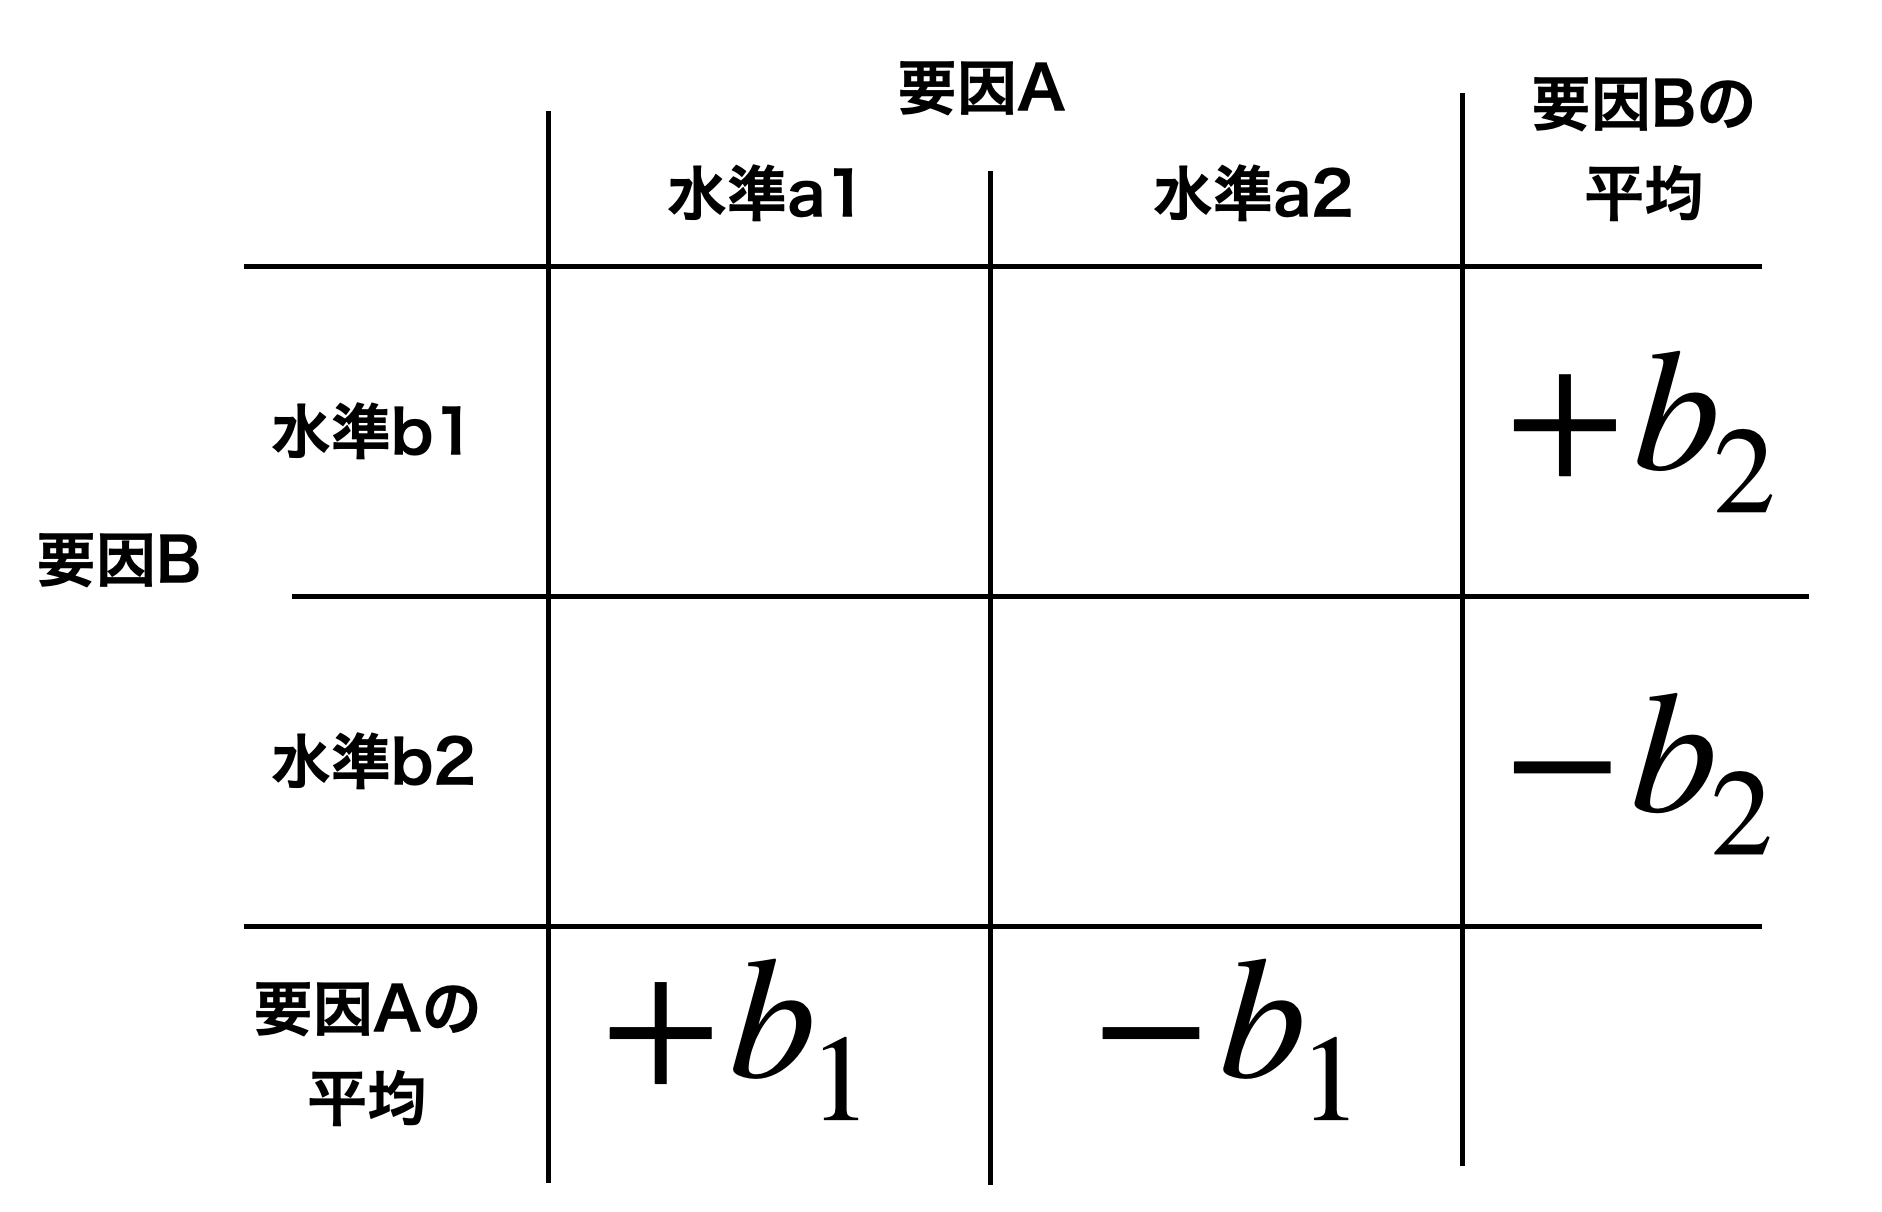
\includegraphics[keepaspectratio,width=0.7\linewidth]{figures/18_BetweenDesign/mainEffect.png}
	\caption{主効果の計算は周辺の平均値から計算する}
	\label{fig:18_03}
\end{figure}

\begin{figure}[ht]
	\centering
	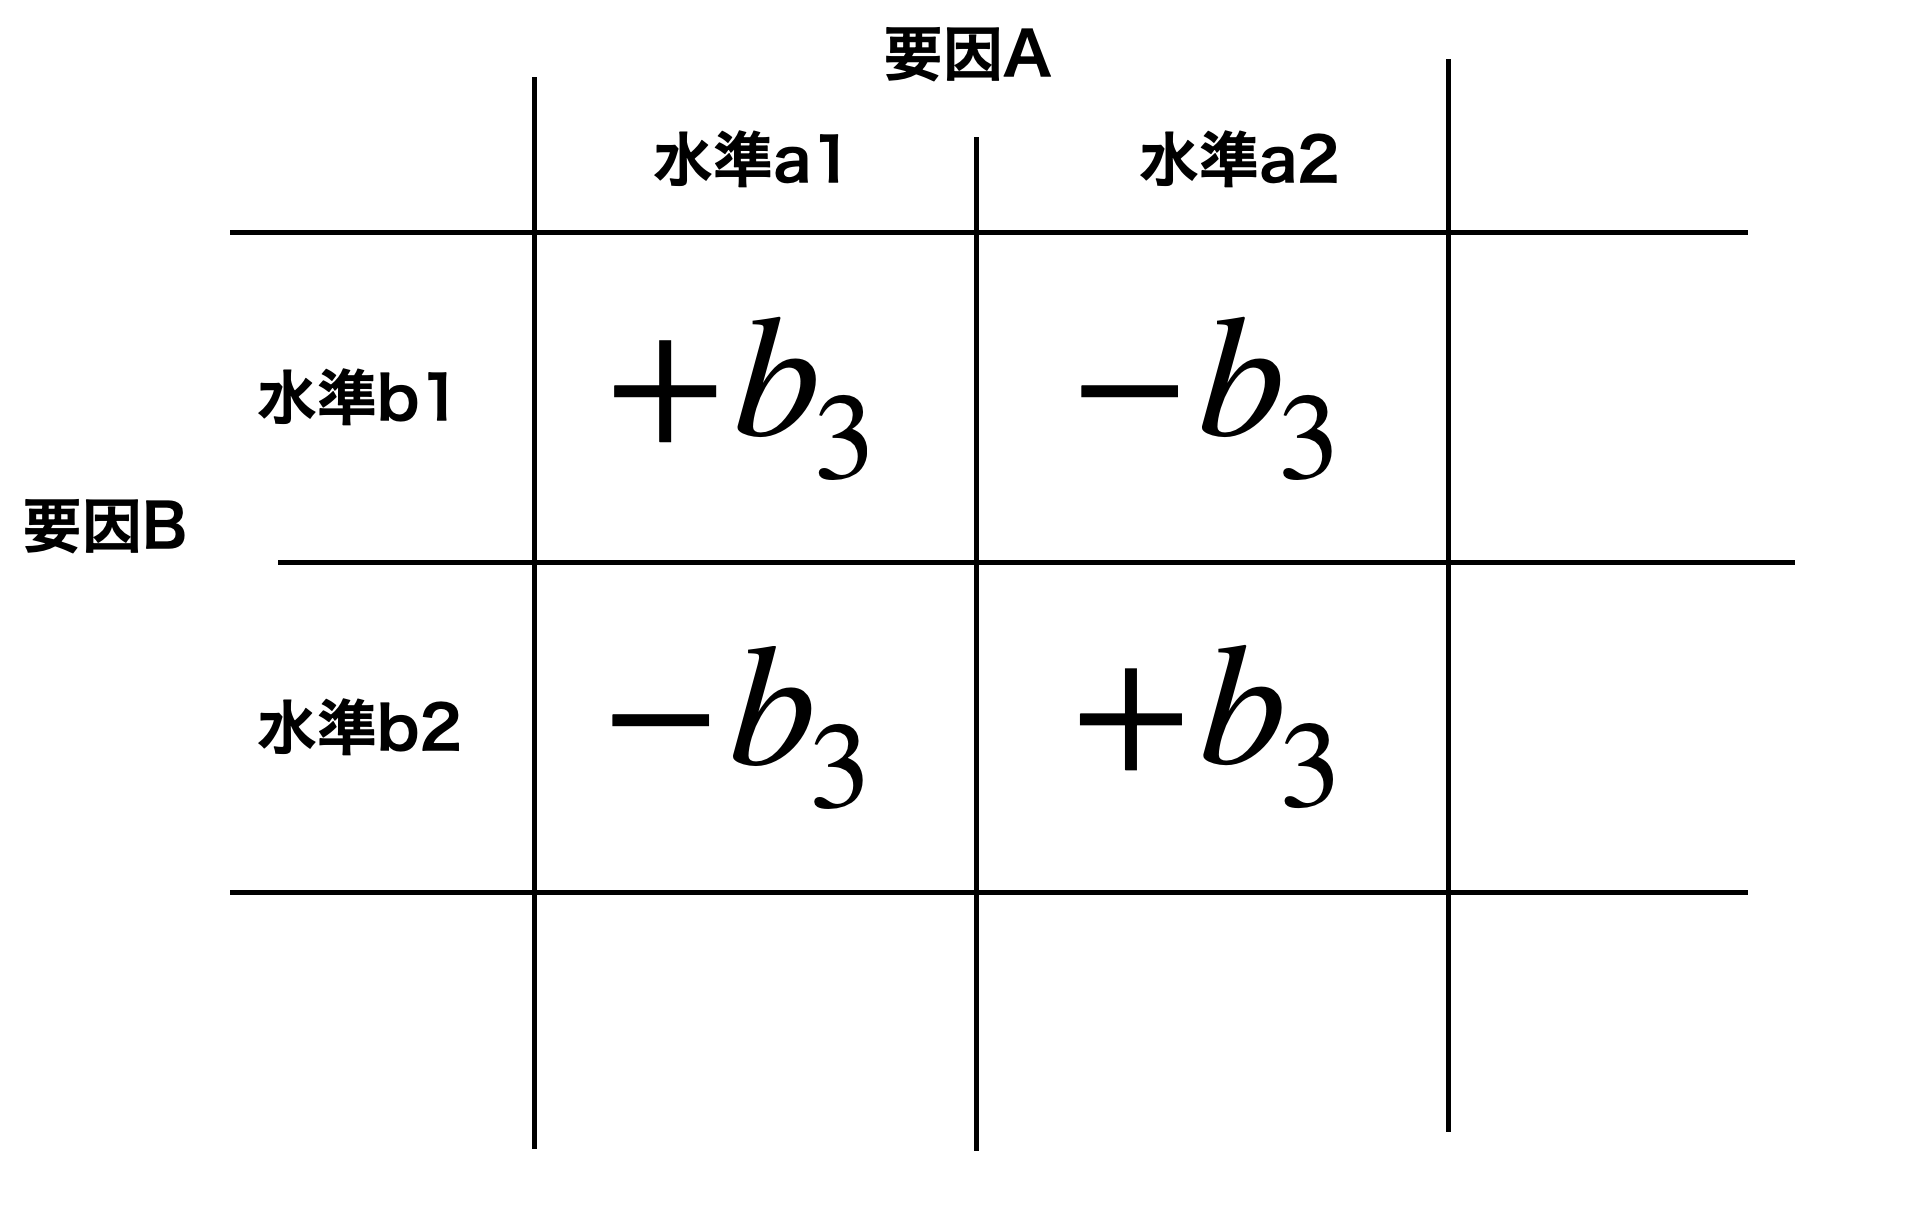
\includegraphics[keepaspectratio,width=0.7\linewidth]{figures/18_BetweenDesign/interaction.png}
	\caption{交互作用はセルの内部で相殺するように}
	\label{fig:18_04}
\end{figure}

このように交互作用を含めて計算すると，組み合わせ水準のところまで含めて，群平均の計算が合うようになります。それでも一人ひとりのレベルまで考えてみると，やはりズレが出てしまいますが，これはどうしようもない個人差＝誤差ですので，これを計算することで誤差を算出できます。

\begin{table}[ht]
	\centering
	\caption{平方和の計算}
	\begin{tabular}{rrrccr}
		\hline
		全体平均 & 温度の効果 & 銘柄の効果 & 交互作用  & 誤差    & 評価    \\
		\hline
		9.75 & -0.25 & +0.75 & +1.75 & +1.00 & 13    \\
		9.75 & -0.25 & +0.75 & +1.75 & -1.00 & 11    \\
		9.75 & -0.25 & +0.75 & +1.75 & 0.00  & 12    \\ \hline
		9.75 & -0.25 & -0.75 & -1.75 & 0.00  & 7     \\
		9.75 & -0.25 & -0.75 & -1.75 & -1.00 & 6     \\
		9.75 & -0.25 & -0.75 & -1.75 & +1.00 & 8     \\ \hline
		9.75 & +0.25 & +0.75 & -1.75 & 0.00  & 9     \\
		9.75 & +0.25 & +0.75 & -1.75 & 0.00  & 9     \\
		9.75 & +0.25 & +0.75 & -1.75 & 0.00  & 9     \\ \hline
		9.75 & +0.25 & -0.75 & +1.75 & +2.00 & 13    \\
		9.75 & +0.25 & -0.75 & +1.75 & 0.00  & 11    \\
		9.75 & +0.25 & -0.75 & +1.75 & -2.00 & 9     \\
		\hline\hline
		平方和  & 0.75  & 6.75  & 36.75 & 12.00 & 56.25 \\\hline
	\end{tabular}
	\label{tbl:18_04}
\end{table}
表\ref{tbl:18_04}には，それぞれの効果の大きさと，それを二乗して足したものを書きました。二乗して足し合わせたものはとくに\keyterm{平方和}{へいほうわ}{sum of squares; SS}といいます。これはもちろん，大きさを比較するために幅の計算にするためです。評価の列にも平方和がありますが，これは各評価と全体平均の差の平方和になっています。評価の平方和はデータ全体のばらつきを表していますが，この全体平方和＝温度効果の平方和＋銘柄の平方和＋交互作用の平方和＋誤差の平方和となっているのがわかります($56.25=0.75+6.75+36.75+12.00$です)。2要因計画の場合も，交互作用を考慮して，データの散らばりを足し算の形に分解できました。

\subsection{交互作用のパターン}
もう一度冒頭の図\ref{fig:18_01}にもどって，2水準$\times$2水準のスコアをそれぞれ見てみましょう。横軸は温度の2水準で，名義尺度水準の数字すなわち離散的な変数ですから適切ではないのですが，同じ条件のところを線で結んでみますとクロスしているのがみて取れると思います(図\ref{fig:18_05})。交互作用が見られる典型的なパターンの1つが，このように平均点を結ぶとクロスする形になります。

\begin{figure}[ht]
	\centering
	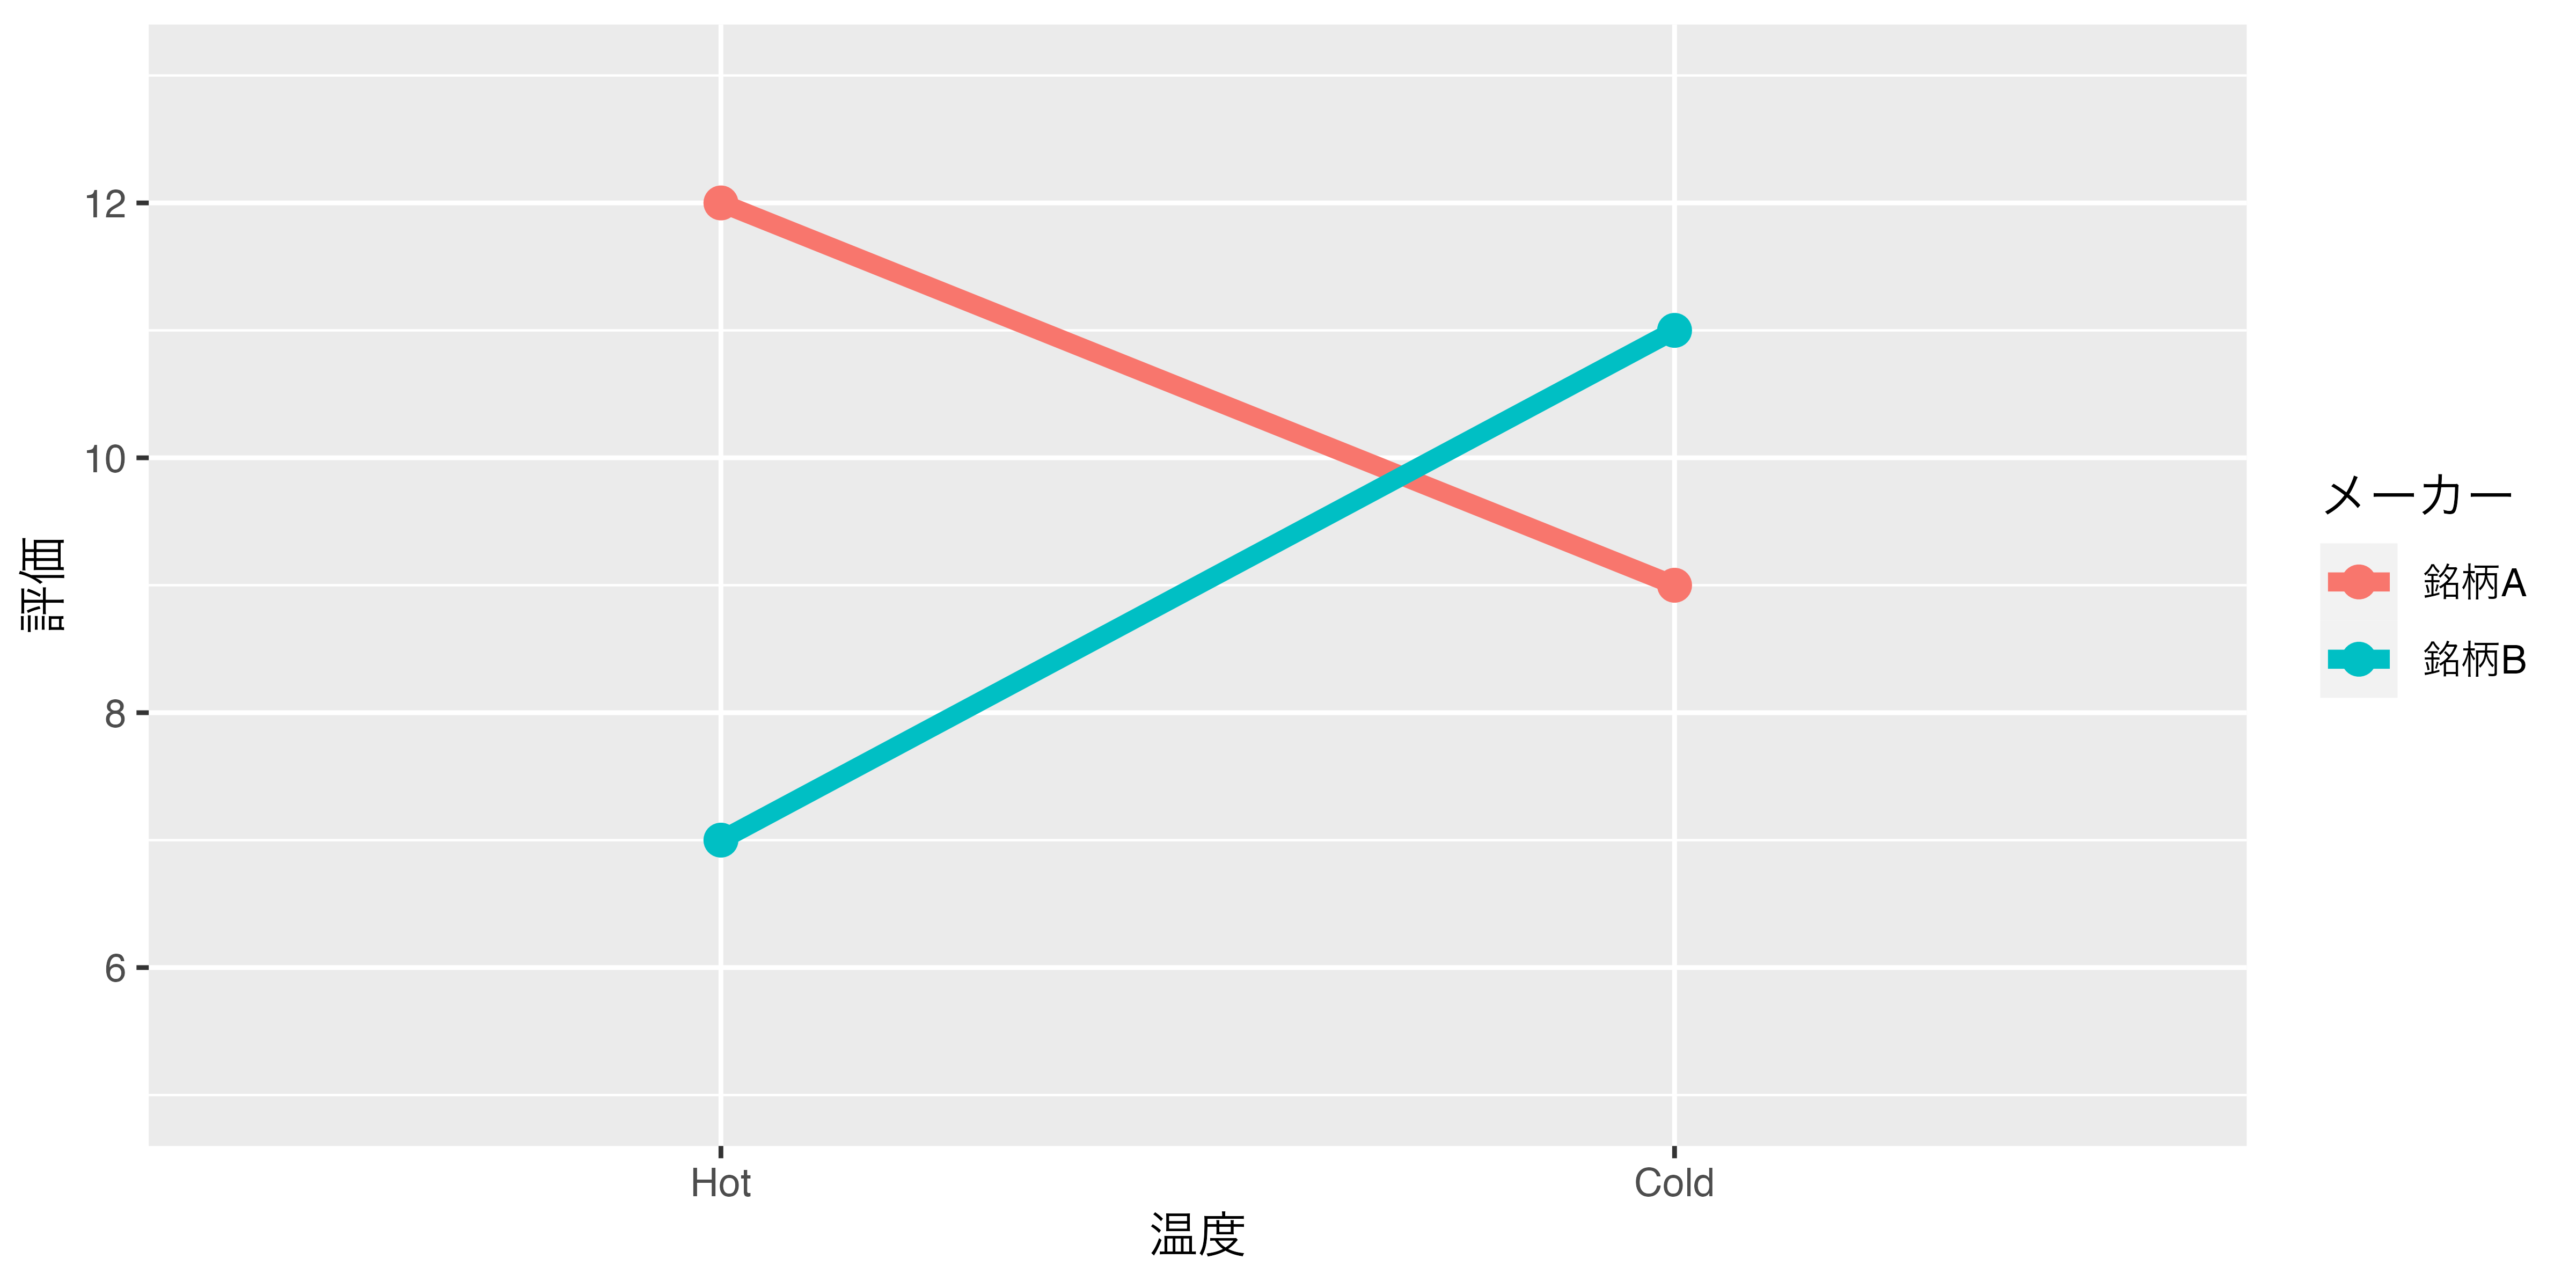
\includegraphics[keepaspectratio,width=0.8\linewidth]{figures/18_BetweenDesign/interaction_pattern1.png}
	\caption{平均点を結ぶとクロスする}
	\label{fig:18_05}
\end{figure}

ここで再確認ですが，主効果というのは各群の平均における差を見るものです。温度の効果を見るときはメーカーの水準に関係なく，温度のHot/Coldの別だけに注目して平均を見ます。
逆にメーカーの効果を見るときは，温度の水準に関係なく銘柄A/Bの違いを見ます。図\ref{fig:18_06}には先ほどのクロスしたラインに主効果の位置を書き加えました。
図\ref{fig:18_06}の左にあるのが，温度の主効果を比べる時の点で，右にあるのがメーカーの主効果を見るときの場所です。主効果はこのように，それ以外の群の水準を潰して平均を見ているわけですね。図\ref{fig:18_03}のように，表で理解した方がわかりやすい人もいるかもしれませんが，表でピンとこなかった人は図でイメージしてみてください。

\begin{figure}[ht]
	\centering
	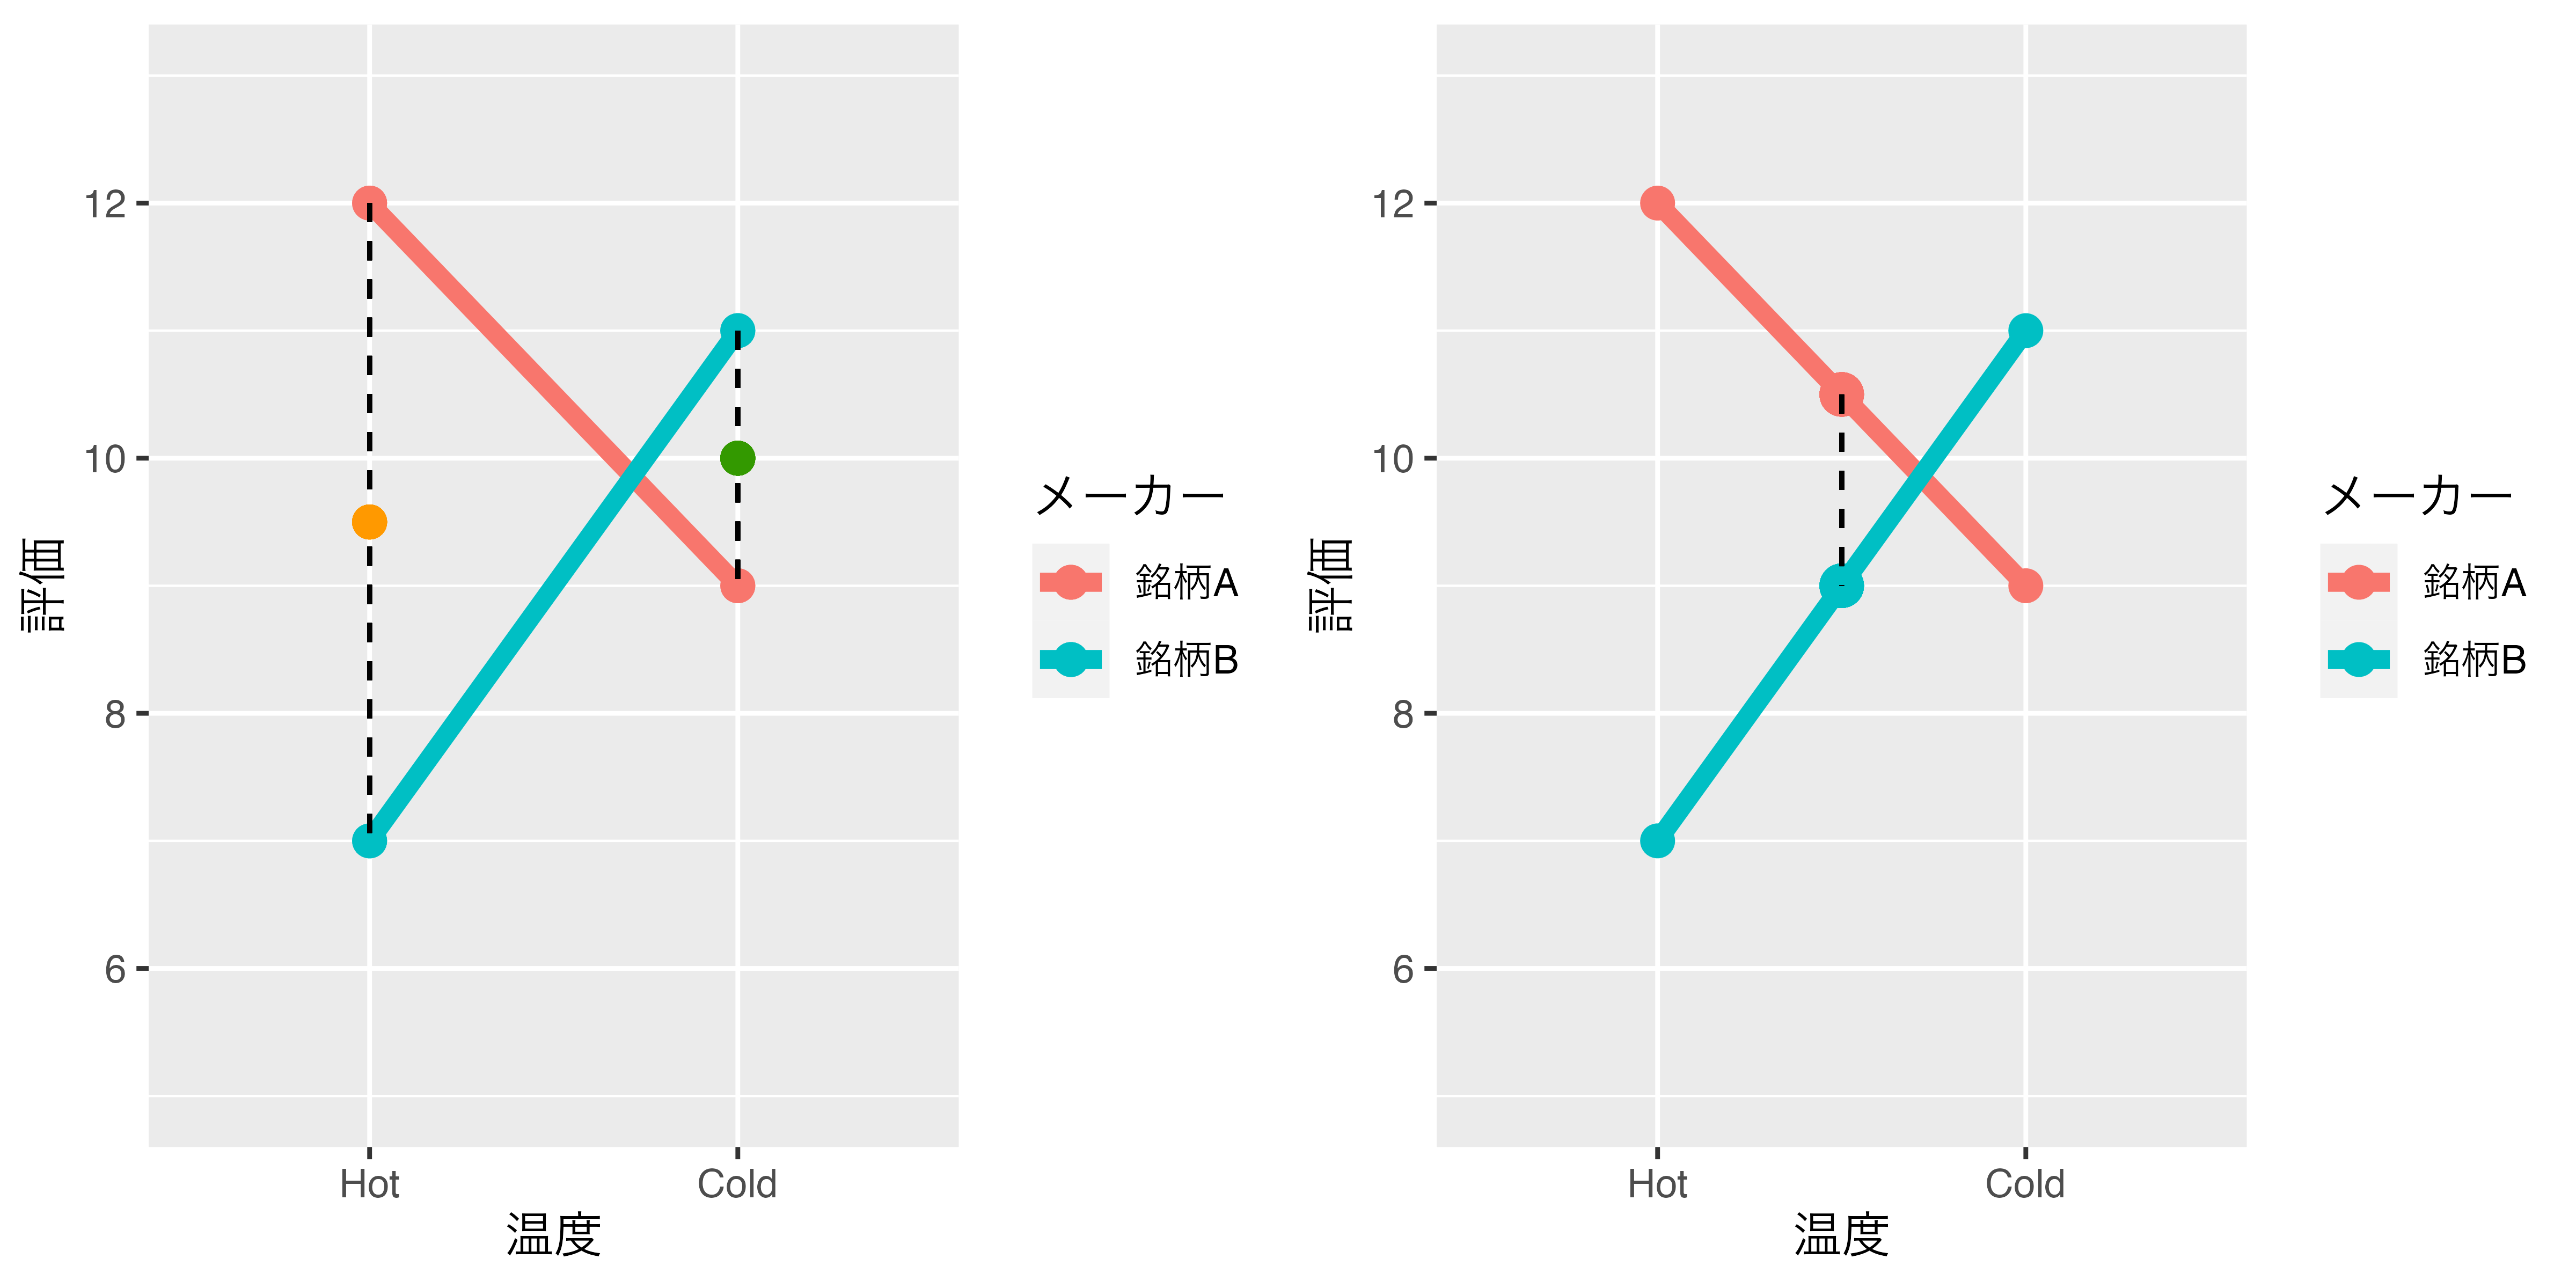
\includegraphics[keepaspectratio,width=0.8\linewidth]{figures/18_BetweenDesign/where_effects_is.png}
	\caption{主効果はどこを比べているのか確認しておこう}
	\label{fig:18_06}
\end{figure}

ところで，交互作用は必ずしもこのクロスしたような状況だけを指すものではありません。基本的に主効果ではなく，組み合わせた時に初めてみられる効果のことを言いますから，交互作用の現れ方は他にもあり得ます。順にいろいろなパターンを見てみましょう。

まず要因A,Bそれぞれの主効果があり，交互作用がない例が図\ref{MainOnly}です。要因Aの第一，第二水準の間に差があるので要因Aの主効果がありますし，要因Bのみ，つまり左右で見比べてもその平均に違いがあります。

一方の要因しか効果がない場合が図\ref{factorAonly},\ref{factorBonly}です。図\ref{factorAonly}は上下の違いだけで左右に違いがありませんから，要因Aの効果だけが出ていることになります。図\ref{factorBonly}は左側と右側の違いがありますが，要因Aの水準に違いがありません。またこの図には交互作用が入っておらず，組み合わせの効果がないのでパターンが比較的みやすくなっています。

図\ref{AllEffects}には，主効果も交互作用も含まれている例を示しました。上側・下側の比較でも差がありますし，左側・右側だけでも差があります。さらに左右を結んだ線が平行になっていないということは，特別な組み合わせの効果がどこかに出ていることを意味します。

図\ref{interactionOnly}は，コーヒーテイスティングの例の極端にしたようなパターンです。これは要因Aの第一水準の平均と第二水準の平均を取っても同じ，要因Bのそれも同じなのですが，明らかに効果の現れ方が一方向的ではありませんね。それぞれの主効果がないのに，交互作用だけあるというパターンです。

\begin{figure}[ht]
	\begin{tabular}{cc}
		\centering
		\begin{minipage}[t]{0.45\hsize}
			\centering
			\begin{tikzpicture}
				\coordinate (A1B1) at (40pt,100pt);
				\coordinate (A1B2) at (100pt,70pt);
				\coordinate (A2B1) at (40pt,70pt);
				\coordinate (A2B2) at (100pt,40pt);
				\draw (0,0)--(0,130pt);
				\draw (0,0)--(130pt,0);
				\coordinate[label=below:B1] (B1) at (40pt,0);
				\coordinate[label=below:B2] (B2) at (100pt,0);
				\draw[] (A1B1)--(A1B2);
				\draw[dashed] (A2B1)--(A2B2);
				\coordinate[label=below:A1] (A1) at (70pt,100pt);
				\coordinate[label=below:A2] (A2) at (70pt,50pt);
				\foreach \P in {A1B1,A1B2,A2B1,A2B2,B1,B2} \fill[black] (\P) circle (0.06);
			\end{tikzpicture}
			\caption{両要因の主効果だけがある}
			\label{MainOnly}
		\end{minipage} &
		\begin{minipage}[t]{0.45\hsize}
			\centering
			\begin{tikzpicture}
				\coordinate (A1B1) at (40pt,100pt);
				\coordinate (A1B2) at (100pt,100pt);
				\coordinate (A2B1) at (40pt,50pt);
				\coordinate (A2B2) at (100pt,50pt);
				\draw (0,0)--(0,130pt);
				\draw (0,0)--(130pt,0);
				\coordinate[label=below:B1] (B1) at (40pt,0);
				\coordinate[label=below:B2] (B2) at (100pt,0);
				\draw[] (A1B1)--(A1B2);
				\draw[dashed] (A2B1)--(A2B2);
				\coordinate[label=below:A1] (A1) at (70pt,100pt);
				\coordinate[label=below:A2] (A2) at (70pt,50pt);
				\foreach \P in {A1B1,A1B2,A2B1,A2B2,B1,B2} \fill[black] (\P) circle (0.06);
			\end{tikzpicture}
			\caption{要因Aの主効果だけがある}
			\label{factorAonly}
		\end{minipage} \\\\

		\begin{minipage}[t]{0.45\hsize}
			\centering
			\begin{tikzpicture}
				\coordinate (A1B1) at (40pt,75pt);
				\coordinate (A1B2) at (100pt,45pt);
				\coordinate (A2B1) at (40pt,70pt);
				\coordinate (A2B2) at (100pt,40pt);
				\draw (0,0)--(0,130pt);
				\draw (0,0)--(130pt,0);
				\coordinate[label=below:B1] (B1) at (40pt,0);
				\coordinate[label=below:B2] (B2) at (100pt,0);
				\draw[] (A1B1)--(A1B2);
				\draw[dashed] (A2B1)--(A2B2);
				\coordinate[label=below:A1] (A1) at (70pt,80pt);
				\coordinate[label=below:A2] (A2) at (70pt,50pt);
				\foreach \P in {A1B1,A1B2,A2B1,A2B2,B1,B2} \fill[black] (\P) circle (0.06);
			\end{tikzpicture}
			\caption{要因Bの主効果だけがある}
			\label{factorBonly}
		\end{minipage} &
		\begin{minipage}[t]{0.45\hsize}
			\centering
			\begin{tikzpicture}
				\coordinate (A1B1) at (40pt,100pt);
				\coordinate (A1B2) at (100pt,90pt);
				\coordinate (A2B1) at (40pt,70pt);
				\coordinate (A2B2) at (100pt,40pt);
				\draw (0,0)--(0,130pt);
				\draw (0,0)--(130pt,0);
				\coordinate[label=below:B1] (B1) at (40pt,0);
				\coordinate[label=below:B2] (B2) at (100pt,0);
				\draw[] (A1B1)--(A1B2);
				\draw[dashed] (A2B1)--(A2B2);
				\coordinate[label=below:A1] (A1) at (70pt,110pt);
				\coordinate[label=below:A2] (A2) at (70pt,50pt);
				\foreach \P in {A1B1,A1B2,A2B1,A2B2,B1,B2} \fill[black] (\P) circle (0.06);
			\end{tikzpicture}
			\caption{主効果も交互作用もある}
			\label{AllEffects}
		\end{minipage} \\ \\
		\multicolumn{2}{c}{
			\begin{minipage}[t]{0.45\hsize}
				\centering
				\begin{tikzpicture}
					\coordinate (A1B1) at (40pt,100pt);
					\coordinate (A1B2) at (100pt,40pt);
					\coordinate (A2B1) at (40pt,40pt);
					\coordinate (A2B2) at (100pt,100pt);
					\draw (0,0)--(0,130pt);
					\draw (0,0)--(130pt,0);
					\coordinate[label=below:B1] (B1) at (40pt,0);
					\coordinate[label=below:B2] (B2) at (100pt,0);
					\draw[] (A1B1)--(A1B2);
					\draw[dashed] (A2B1)--(A2B2);
					\coordinate[label=below:A1] (A1) at (50pt,110pt);
					\coordinate[label=below:A2] (A2) at (60pt,50pt);
					\foreach \P in {A1B1,A1B2,A2B1,A2B2,B1,B2} \fill[black] (\P) circle (0.06);
				\end{tikzpicture}
				\caption{主効果はないが交互作用だけがある}
				\label{interactionOnly}
			\end{minipage}
		}
	\end{tabular}

\end{figure}

今回のコーヒーテイスティング事例では，主効果の大きさよりも大きさの方が強かったので，図\ref{interactionOnly}のような形になったのでしょう。実際に「どれぐらい大きければ意味があるのか」といったことについては，後期の推測統計学に入ってから学ぶことになります。そこでは効果の大きさを評価し，意味があるのかどうかを判断するということについて学びますが，今のところはひとまず算出方法と，出現パターンのあり方について把握しておいてください。何にせよ，\textbf{データは図にする}ことの重要性が，改めて分かったのではないかと思います。


\subsection{組み合わせが増えると}
ところで今回，要因の組み合わせによる影響，つまり交互作用を考えようという話でした。今回は2要因の例でしたが，3要因になるとさらにその組み合わせは増えます。下に要因計画ごとの要素の組み合わせを書いてみました。
\[
	\begin{array}{llll}
		\mbox{一要因群間計画} & \mbox{全体変動} & = & \mbox{要因A} + \mbox{誤差}                                                          \\
		\mbox{一要因群内計画} & \mbox{全体変動} & = & \mbox{要因A} + \mbox{個人差} + \mbox{誤差}                                             \\
		\mbox{二要因群間計画} & \mbox{全体変動} & = & \mbox{要因A} + \mbox{要因B} +\mbox{交互作用AB} +\mbox{誤差}                               \\
		\mbox{三要因群間計画} & \mbox{全体変動} & = & \mbox{要因A} + \mbox{要因B} + \mbox{要因C}+\mbox{交互作用AB} +\mbox{交互作用AC}+\mbox{交互作用BC} \\
		               &             &   & +\mbox{交互作用ABC}  +\mbox{誤差}                                                     \\
		\mbox{四要因群間計画} & \mbox{全体変動} & = & \mbox{要因A} + \mbox{要因B} + \mbox{要因C} + \mbox{要因D}                               \\
		               &             &   & + \mbox{交互作用AB} +\mbox{交互作用AC} +\mbox{交互作用AD}+\mbox{交互作用BC}                     \\
		               &             &   & +\mbox{交互作用BD} +\mbox{交互作用CD}+\mbox{交互作用ABC}+\mbox{交互作用ABD}                     \\
		               &             &   & +\mbox{交互作用BCD} +\mbox{交互作用ABCD} +\mbox{誤差}                                     \\
	\end{array}
\]
3要因になると，3つの主効果(効果A,B,C)に加え，組み合わせの効果がAB,AC,BCの一次の交互作用だけでなく，ABC3つ揃った時の二次の交互作用も考える必要があります。4要因についても書いてみましたが，もう訳が分からないレベルです。

このことからわかるように，要因計画はいくらでも複雑にしても良い，というものではありません。要因が増えるごとに考えるべき要素が増えるだけであり，結局統一的な解釈が難しくなります。お勧めとしては，交互作用のないような現象について，二要因までの研究計画にしておいた方が良いように思います。

\section{課題}

\subsection{問題1：効果の大きさの算出}

ある研究者が，勉強時間（長い・短い）と睡眠時間（十分・不足）がテストの点数に与える影響を調べるため，$2\times2$の群間計画で実験を行いました。各条件に4名ずつ配置し，100点満点のテストを実施したところ，各群の平均点は表\ref{tbl:18_05}のようになりました。

\begin{table}[ht]
	\centering
	\caption{勉強時間と睡眠時間によるテスト成績}
	\begin{tabular}{c|cc}
		          & 勉強時間：長い & 勉強時間：短い \\ \hline
		睡眠：十分 & 80点        & 60点        \\
		睡眠：不足 & 65点        & 55点        \\ \hline
	\end{tabular}
	\label{tbl:18_05}
\end{table}

この時，次の値を算出しなさい。

\begin{enumerate}
	\item 全体平均（Grand Mean）
	\item 勉強時間の主効果の大きさ（$|b_1|$）
	\item 睡眠時間の主効果の大きさ（$|b_2|$）
	\item 交互作用の効果の大きさ（$|b_3|$）
\end{enumerate}

ただし，効果の大きさは「群平均 - 全体平均」で表現できます。また，勉強時間が長い条件を$+1$，短い条件を$-1$，睡眠が十分な条件を$+1$，不足の条件を$-1$としてコーディングします。

\subsection{問題2：平方和の計算}

表\ref{tbl:18_06}は，ある二要因実験（各セル3名）の結果です。

\begin{table}[ht]
	\centering
	\caption{実験データ}
	\begin{tabular}{cccc}
		\hline
		要因A  & 要因B  & データ          & 平均   \\ \hline
		$a_1$ & $b_1$ & 12, 14, 13   & 13.0 \\
		$a_1$ & $b_2$ & 8, 10, 9     & 9.0  \\
		$a_2$ & $b_1$ & 10, 12, 11   & 11.0 \\
		$a_2$ & $b_2$ & 14, 16, 15   & 15.0 \\ \hline
	\end{tabular}
	\label{tbl:18_06}
\end{table}

次の値を算出しなさい。

\begin{enumerate}
	\item 全体平均
	\item 要因Aの主効果（$b_1$）
	\item 要因Bの主効果（$b_2$）
	\item 交互作用（$b_3$）
	\item 各効果の平方和（SS）
\end{enumerate}

ただし，要因Aは$a_1$を$+1$，$a_2$を$-1$とし，要因Bは$b_1$を$+1$，$b_2$を$-1$としてコーディングします。

\end{document}
